\documentclass{beamer}

\usepackage[utf8]{inputenc}
\usepackage[T1]{fontenc}

\usepackage[english]{babel}
\usepackage{amsmath}
\usepackage{cleveref}
\usepackage{amssymb}
\usepackage{mathtools}

%%Numbers, expectation
\newcommand{\N}{\mathbb{N}}
\newcommand{\E}{\mathbb{E}}
\renewcommand{\P}{\mathbb{P}}
\newcommand{\Var}{\mathbb{V}}
\newcommand{\R}{\mathbb{R}}
\newcommand{\D}{\mathcal{D}}
\newcommand{\B}{\mathcal{B}}
\newcommand{\Dh}{\D_h}
\renewcommand{\phi}{\varphi}
\newcommand*\diff{\mathop{}\!\mathrm{d}} % integral

%% mathoperator
\DeclareMathOperator*{\argmax}{arg\,max}
\DeclareMathOperator*{\argmin}{arg\,min}
\DeclareMathOperator*{\dom}{dom}
\DeclareMathOperator*{\sign}{sign}
\DeclareMathOperator*{\diag}{diag}

\DeclareMathOperator*{\Cov}{Cov}
\DeclareMathOperator*{\Cor}{Corr}
\DeclareMathOperator*{\Id}{Id}

%proximal operator
\newcommand{\prox}[3][]{\operatorname{prox}^{#1}_{#2}\left(#3 \right)}

\usepackage{xcolor}

%% sort citations by increasing number
\usepackage[sort,nocompress]{cite}

\usepackage{graphicx}% http://ctan.org/pkg/graphicx
\graphicspath{{../figures/}{../../figures}{../../memes}} %Setting the graphicspath
\usepackage{caption,subcaption}

\usepackage{tikz}
\usepackage{pgfplots}
\usetikzlibrary{backgrounds}
\usetikzlibrary{intersections}
\usepgfplotslibrary{fillbetween}

% \usepackage[right]{showlabels}


%%
\theoremstyle{plain}
\newtheorem{prop}{Proposition}[section]
\newtheorem{algo}{Algorithm}[section]
\newtheorem{assumption}{Assumption}
\theoremstyle{remark}
\newtheorem{remark}{Remark}[section]

% cref
\crefname{assumption}{Assumption}{Assumptions}
\crefname{equation}{}{}

\usepackage{autonum}

\usepackage{bm} %% bold math symbols

\usepackage{bbm} %% for \mathbbm{1}


% algorithmic environment
\usepackage{algorithm}
\usepackage[noend]{algpseudocode}

% for some reason this was required on one void linux installation (but not the other)
\usepackage{sansmathaccent}
\pdfmapfile{+sansmathaccent.map}

\author{Axel Böhm}

% shows which section we're in
\usetheme{Darmstadt}

% page number
\setbeamertemplate{footline}[frame number]
\setbeamercolor{page number in head/foot}{fg=gray}


% display things like onslide or visible already before but grayed out
\setbeamercovered{transparent}

% set the itemize item symbol as a diamond
\setbeamertemplate{itemize item}{$\diamond$}
% set the itemize subitem symbol as a triangle
\setbeamertemplate{itemize subitem}{$\blacktriangleright$}

% set the enumerate item symbol as a roman numbers
\setbeamertemplate{enumerate item}{(\roman{enumi})}

\DeclareMathOperator*{\perm}{perm}

\title{Matrix games}
\date{\today}

\begin{document}
\maketitle
\frame{\tableofcontents[currentsection]}

\section{Introduction}%

\begin{frame}
  \frametitle{Introduction}
  Given
  \begin{itemize}
    \item Player I (rows, Alice)
          \item Player II (columns, Bob)
          \item a \emph{payoff} matrix $A \in \R^{m \times n}$
  \end{itemize}
  Every round
  \begin{enumerate}
    \item Alice picks (row) strategy $i\in [m]:= \{1,\dots, m\}$
          Bob picks (col) strategy $j\in [n]$
    \item Bob pays Alice the amount $a_{i,j}$
  \end{enumerate}
  \begin{center}
    \textbf{zero-sum game}
  \end{center}
\end{frame}

\begin{frame}
  \frametitle{Example: penalty game}
  \begin{figure}[ht]
    \centering
    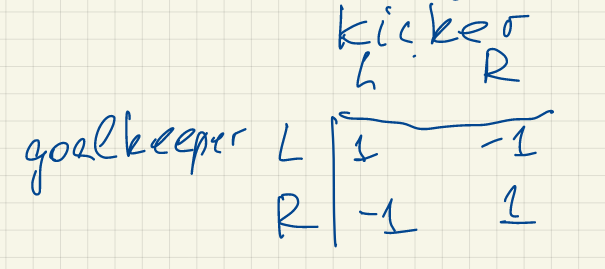
\includegraphics[scale=0.2]{penalty-game.png}
    \caption{penalty game}
  \end{figure}
\end{frame}

\begin{frame}
  \frametitle{Example: prisoners dilemma}
  \begin{figure}[ht]
    \centering
    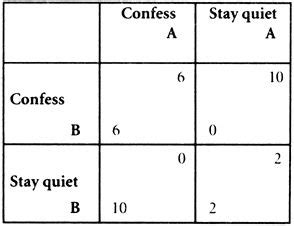
\includegraphics[width=0.5\textwidth]{prison.jpg}
    \caption{\label{fig:label} }
  \end{figure}
\end{frame}

\begin{frame}
  \frametitle{Worst case}

  \begin{itemize}
    \item Alice gets $\onslide<2->{\max_{j\in [m]}}\min_{j\in [n]} a_{i,j}$
    \onslide<3->{\item Bob gets $\min_{j\in [n]} \max_{j\in [m]} a_{i,j}$}
  \end{itemize}
  \onslide<4->{%
    We claim:
    \begin{equation}
      \max_i \min_j a_{i,j} \le \min_{j} \max_i a_{i,j}
    \end{equation}
    \begin{center}
      \textit{``Tallest dwarf is not as tall as the smallest giant.''}
    \end{center}
    But equality does not hold in general!
  }
  % \begin{proof}
  %   lala
  % \end{proof}
\end{frame}

\begin{frame}
  \frametitle{Proof of the min-max theorem}
  \begin{equation}
    \begin{aligned}
      a_{ij} &\le a_{ij} & \forall i,j \\
      \onslide<2->{a_{ij} &\le \max_i a_{ij} & \forall i,j }\\
      \onslide<3->{\min_j a_{ij} &\le \min_j \max_i a_{ij} & \forall i}\\
    \end{aligned}
  \end{equation}
  \onslide<4->{%
  \begin{definition}
    We call $(i^*, j^*)$ a saddle point (or \emph{Nash equilibrium}) if
    \begin{equation}
      \max_i a_{ij^*} = a_{i^*j^*} = \min_j a_{i^*j}.
    \end{equation}
    These are called \emph{pure strategies}.
  \end{definition}
  }
\end{frame}

% Talk about stackelberg?

\begin{frame}
  \frametitle{Rock paper scissors}
  \begin{equation}
    \begin{array}{l|ccc}
        & R & P & S \\
      \hline
      R & 0 & -1 & 1 \\
      P & 1 & 0 & -1 \\
      S & -1 & 1 & 0
    \end{array}
  \end{equation}
\end{frame}

\begin{frame}
  \frametitle{Mixed Strategies}
  With pure strategies we do not always have a saddle point.
  \begin{block}{von Neumann (1928) --- Mixed strategies}
    \begin{itemize}
      \item Alice picks strategies $1, \dots, m$ \emph{with probabilities} $x\in \Delta_m$
      \item Bob picks strategies $1, \dots, n$ \emph{with probabilities} $x\in \Delta_n$
    \end{itemize}
    Expected gain of Alice is
    \begin{equation}
      \langle x, Ay \rangle = \sum_{i,j} a_{ij} x_i y_j
    \end{equation}
  \end{block}
  \onslide<2->{%
    \begin{theorem}{Saddle point exists}
      Expected gain of Alice $=$ expected loss of Bob
      \begin{equation}
        \max_{x \in \Delta} \min_{y \in \Delta} \langle x, Ay \rangle = \min_{y \in \Delta} \max_{x \in \Delta} \langle x, Ay \rangle.
      \end{equation}

    \end{theorem}
  }
\end{frame}

\section{Algorithms}%
\label{sec:}

\begin{frame}
  \frametitle{Stopping criteria}
  \begin{equation}
    \begin{aligned}
      \min_{x \in \Delta} \max_{y \in \Delta} \langle x, Ay \rangle =: v \\
      \max_{y \in \Delta} \min_{x \in \Delta} \langle x, Ay \rangle = v
    \end{aligned}
  \end{equation}
  \begin{block}{stopping criterion}
    \begin{equation}
      \begin{aligned}
        f_p(x) - f_p(x^*) &= f_p(x) - v \onslide<2->{\textcolor{red}{\, \le \epsilon/2}}\\
        f_d(y^*) - f_d(y) &= v - f_d(y) \onslide<2->{\textcolor{red}{\, \le \epsilon/2}} \\
        \onslide<3->{\Rightarrow f_p(x) - f_d(y) \le \epsilon}
      \end{aligned}
    \end{equation}
  \end{block}
  \begin{center}
    Before we never had the optimal value!
  \end{center}
  Solution will always be on the boundary:
  \begin{equation}
    f_p(x) = \max_{y \in \Delta} \langle A^T x, y \rangle = \max_{j} \langle A^T x, e_j \rangle
  \end{equation}
\end{frame}


\begin{frame}
  \frametitle{}
  Consider
  \begin{equation}
      \min_{x \in \Delta} \max_{y \in \Delta} \langle x, Ay \rangle
  \end{equation}
  as a minimization problem
  \begin{equation}
      \min_{x \in \Delta} \langle x, A y^* \rangle
  \end{equation}
  Then
  \begin{equation}
    x^* \in \argmin_{y \in \Delta} f_p(x)  \Leftrightarrow \langle \nabla f_p(x^*), x-x^* \rangle \ge 0 \quad \forall x \in D
  \end{equation}
  Thus
  \begin{equation}
    \begin{aligned}
      \langle A^T y^*, x-x^* \rangle &\ge 0 \quad \forall  x \in D \\
      \langle -A x^*, y-y^* \rangle &\ge 0 \quad \forall  y \in D \\
    \end{aligned}
  \end{equation}
  Concatenate the two conditions to get
  \begin{equation}
  \left\langle \begin{bmatrix}
      0 & A^T \\
      -A & 0
    \end{bmatrix}
    \left(\begin{array}{c}
      x^*\\ y^*
    \end{array}  \right),
    \left(\begin{array}{c}
      x \\ y
    \end{array}  \right)
    -
    \left(\begin{array}{c}
      x^* \\
      y^*
    \end{array} \right)
 \right\rangle
  \end{equation}

\end{frame}

\begin{frame}
  \frametitle{}
  By rewriting $z=(x,y)$ and $F(z) = [A^T y; Ax]$, then
  \begin{equation}\tag{VI}
    \label{eq:VI}
    \langle F(z^*), z-z^* \rangle \ge 0 \quad \forall z \in \Delta_n \times \Delta_m := C
  \end{equation}
  \begin{center}
    \textbf{Variational inequality}
  \end{center}

  If $F = \nabla \phi$ then~\eqref{eq:VI} would be equivalent to
  \begin{equation}
    \min_C \phi
  \end{equation}


\end{frame}


\end{document}
